\begin{enumialphparenastyle}

\begin{ex} Find $-3\begin{mymatrix}{r}
5 \\
-1 \\
2 \\
-3
\end{mymatrix} +5\begin{mymatrix}{r}
-8 \\
2 \\
-3 \\
6
\end{mymatrix} .$ 
\begin{sol}
$\begin{mymatrix}{r}
-55 \\
13 \\
-21 \\
39
\end{mymatrix}$
\end{sol}
\end{ex}

\begin{ex} Find $-7\begin{mymatrix}{r}
6 \\
0 \\
4 \\
-1
\end{mymatrix} +6\begin{mymatrix}{r}
-13 \\
-1 \\
1 \\
6
\end{mymatrix} .$ 
%\begin{sol}
%\end{sol}
\end{ex}


\begin{ex}
Decide whether 
\begin{equation*}
\vect{v}= \begin{mymatrix}{r}
4 \\
4 \\
-3
\end{mymatrix}
\end{equation*}
is a linear combination of the vectors 
\begin{equation*}
\vect{u}_1 = \begin{mymatrix}{r}
3 \\
1 \\
-1
\end{mymatrix}
\mbox{ and } 
\vect{u}_2 = 
\begin{mymatrix}{r}
2 \\
-2\\
1
\end{mymatrix}.
\end{equation*}

\begin{sol}
\begin{equation*}
\begin{mymatrix}{r}
4 \\
4 \\
-3
\end{mymatrix}
=
2
\begin{mymatrix}{r}
3 \\
1 \\
-1
\end{mymatrix}
-
\begin{mymatrix}{r}
2 \\
-2\\
1
\end{mymatrix}
\end{equation*}
\end{sol}
\end{ex}


\begin{ex}
Decide whether 
\begin{equation*}
\vect{v}= \begin{mymatrix}{r}
4 \\
4 \\
4
\end{mymatrix}
\end{equation*}
is a linear combination of the vectors 
\begin{equation*}
\vect{u}_1 = \begin{mymatrix}{r}
3 \\
1 \\
-1
\end{mymatrix} , \ 
\vect{u}_2 = 
\begin{mymatrix}{r}
8 \\
0\\
-1
\end{mymatrix}
\mbox{ and } 
\vect{u}_3 = 
\begin{mymatrix}{r}
2 \\
-2\\
1
\end{mymatrix}.
\end{equation*}

\begin{sol}
The system 
\begin{equation*}
\begin{mymatrix}{r}
4 \\
4 \\
4
\end{mymatrix}
=
a_1
\begin{mymatrix}{r}
3 \\
1 \\
-1
\end{mymatrix}
+a_2
\begin{mymatrix}{r}
8 \\
0\\
-1
\end{mymatrix}
+a_3
\begin{mymatrix}{r}
2 \\
-2\\
1
\end{mymatrix}
\end{equation*}
has no solution.
\end{sol}
\end{ex}

\begin{ex}
  Consider the vectors $\vect{u}$ and $\vect{v}$ drawn below. 
  \begin{center}
    \begin{tikzpicture}[scale=2]
      \draw[->, thick, blue] (0,0)--(2,1);
      \draw[->, thick, red] (4,1)--(5,0.5);
      \node[below] at (1,1.25){$\vect{u}$};
      \node[above right] at (4.5, 0.75){$\vect{v}$};
    \end{tikzpicture}
  \end{center}
  Draw  $-\vect{u}$, $2\vect{v}$, and $-\frac{1}{2}\vect{v}$.
  
  \begin{sol}
    ~
    \begin{center}
      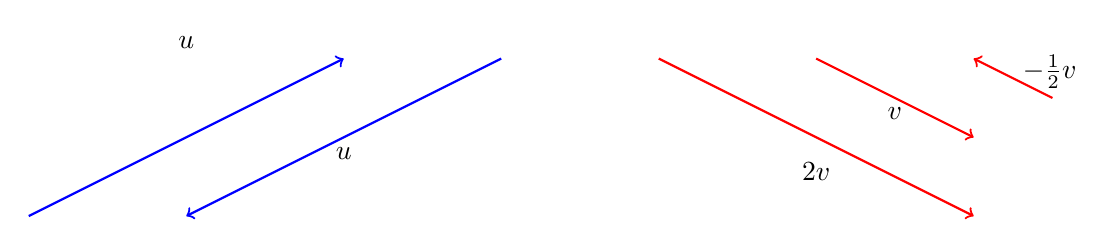
\begin{tikzpicture}[scale=2]
        \draw[->, thick, blue] (0,0)--(2,1);
        \draw[->, thick, blue] (3,1)--(1,0);
        \draw[->, thick, red] (5,1)--(6,0.5);
        \draw[->, thick, red] (6.5,0.75)--(6,1);
        \draw[->, thick, red] (4,1)--(6,0);
        \node[above] at (1,1){$\vect{u}$};
        \node[below] at (2,0.5){$\vect{u}$};
        \node[below] at (5.5, 0.75){$\vect{v}$};
        \node[above right] at (6.25, 0.75){$-\frac{1}{2}\vect{v}$};
        \node[below] at (5, 0.4){$2\vect{v}$};
      \end{tikzpicture}
    \end{center}
  \end{sol}
\end{ex}

\end{enumialphparenastyle}
